\documentclass{article}






\usepackage[preprint]{neurips_2024}






\usepackage[utf8]{inputenc} %
\usepackage[T1]{fontenc}    %
\usepackage{hyperref}       %
\usepackage{url}            %
\usepackage{booktabs}       %
\usepackage{amsfonts}       %
\usepackage{nicefrac}       %
\usepackage{microtype}      %
\usepackage{xcolor}         %
\usepackage{graphicx}
\usepackage{enumitem}
\usepackage{framed}
\usepackage[most]{tcolorbox}
\usepackage{amsmath}

\usepackage{cleveref}
\usepackage{wrapfig}

\usepackage{float}

\usepackage{listings}

\lstset{
  breaklines=true,
  breakatwhitespace=true,
  breakautoindent=false,
  breakindent=0pt,
  basicstyle=\ttfamily    %
}


\newlength{\chatwidth}

\newcommand{\chatbox}[3]{%
    \begingroup
    \setlength{\chatwidth}{#1}%
    \noindent\textbf{User}
    \vspace{-5pt}
    \begin{tcolorbox}[
        colback=white, 
        colframe=black, 
        rounded corners, 
        width=\chatwidth, 
        boxrule=0.2pt,
        left=1mm, right=1mm, top=1mm, bottom=1mm, %
        boxsep=1mm
    ]
        #2
    \end{tcolorbox}
    
    
    \noindent\textbf{Assistant}
    \vspace{-5pt}
    \begin{tcolorbox}[
        colback=white, 
        colframe=black, 
        rounded corners, 
        width=\chatwidth, 
        boxrule=0.2pt,
        left=1mm, right=1mm, top=1mm, bottom=1mm, %
        boxsep=1mm
    ]
        #3
    \end{tcolorbox}
    \endgroup
}


\title{Utility Engineering: Analyzing and Controlling\\Emergent Value Systems in AIs}


\usepackage[affil-it]{authblk}
\usepackage[affil-it]{authblk}
\renewcommand\Authands{, }
\renewcommand\Authfont{\normalfont\bfseries\linespread{2}}
\renewcommand\Affilfont{\normalfont\linespread{1.5}}

\makeatletter \renewcommand\AB@affilsepx{\:  \protect\Affilfont \protect\centering} \makeatother

\newcommand{\printfnsymbol}[1]{%
  \textsuperscript{$\ast$}%
}

\author[1]{Mantas Mazeika}
\author[1]{Xuwang Yin}
\author[1]{Rishub Tamirisa}
\author[2]{Jaehyuk Lim}
\author[2]{\\Bruce W. Lee}
\author[2]{Richard Ren}
\author[1]{Long Phan}
\author[3]{Norman Mu}
\author[1]{\\Adam Khoja}
\author[1]{Oliver Zhang}
\author[1]{Dan Hendrycks}

\affil[1]{Center for AI Safety\par}
\affil[2]{University of Pennsylvania\par}
\affil[3]{University of California, Berkeley}



\usepackage{algorithmic}
\usepackage{algorithm}

\usepackage{caption}

\usepackage{tikz}
\usetikzlibrary{positioning}
\usetikzlibrary{calc}






\begin{document}


\maketitle


\begin{abstract}
Large language model (LLM)-based agents have shown promise in tackling complex tasks by interacting dynamically with the environment. 
Existing work primarily focuses on behavior cloning from expert demonstrations and preference learning through exploratory trajectory sampling. However, these methods often struggle in long-horizon tasks, where suboptimal actions accumulate step by step, causing agents to deviate from correct task trajectories.
To address this, we highlight the importance of \textit{timely calibration} and the need to automatically construct calibration trajectories for training agents. We propose \textbf{S}tep-Level \textbf{T}raj\textbf{e}ctory \textbf{Ca}libration (\textbf{\model}), a novel framework for LLM agent learning. 
Specifically, \model identifies suboptimal actions through a step-level reward comparison during exploration. It constructs calibrated trajectories using LLM-driven reflection, enabling agents to learn from improved decision-making processes. These calibrated trajectories, together with successful trajectory data, are utilized for reinforced training.
Extensive experiments demonstrate that \model significantly outperforms existing methods. Further analysis highlights that step-level calibration enables agents to complete tasks with greater robustness. 
Our code and data are available at \url{https://github.com/WangHanLinHenry/STeCa}.
\end{abstract}

\begin{figure}[!t]
    \centering
    \includegraphics[width=1\textwidth]{figures/Banner_Figures/fig1_new.pdf}
    \caption{Overview of the topics and results in our paper. In \Cref{sec:emergent_value_systems}, we show that coherent value systems emerge in AIs, and we propose the research avenue of Utility Engineering to analyze and control these emergent values. We highlight our utility analysis experiments in \Cref{sec:structural_properties}, a subset of our analysis of salient values held by LLMs in \Cref{sec:salient_values}, and our utility control experiments in \Cref{sec:utility_control}.}
    \label{fig:main_fig}
\end{figure}

\clearpage
{
\hypersetup{linkcolor=black}
\tableofcontents
}
\clearpage


\section{Introduction}

Despite the remarkable capabilities of large language models (LLMs)~\cite{DBLP:conf/emnlp/QinZ0CYY23,DBLP:journals/corr/abs-2307-09288}, they often inevitably exhibit hallucinations due to incorrect or outdated knowledge embedded in their parameters~\cite{DBLP:journals/corr/abs-2309-01219, DBLP:journals/corr/abs-2302-12813, DBLP:journals/csur/JiLFYSXIBMF23}.
Given the significant time and expense required to retrain LLMs, there has been growing interest in \emph{model editing} (a.k.a., \emph{knowledge editing})~\cite{DBLP:conf/iclr/SinitsinPPPB20, DBLP:journals/corr/abs-2012-00363, DBLP:conf/acl/DaiDHSCW22, DBLP:conf/icml/MitchellLBMF22, DBLP:conf/nips/MengBAB22, DBLP:conf/iclr/MengSABB23, DBLP:conf/emnlp/YaoWT0LDC023, DBLP:conf/emnlp/ZhongWMPC23, DBLP:conf/icml/MaL0G24, DBLP:journals/corr/abs-2401-04700}, 
which aims to update the knowledge of LLMs cost-effectively.
Some existing methods of model editing achieve this by modifying model parameters, which can be generally divided into two categories~\cite{DBLP:journals/corr/abs-2308-07269, DBLP:conf/emnlp/YaoWT0LDC023}.
Specifically, one type is based on \emph{Meta-Learning}~\cite{DBLP:conf/emnlp/CaoAT21, DBLP:conf/acl/DaiDHSCW22}, while the other is based on \emph{Locate-then-Edit}~\cite{DBLP:conf/acl/DaiDHSCW22, DBLP:conf/nips/MengBAB22, DBLP:conf/iclr/MengSABB23}. This paper primarily focuses on the latter.

\begin{figure}[t]
  \centering
  \includegraphics[width=0.48\textwidth]{figures/demonstration.pdf}
  \vspace{-4mm}
  \caption{(a) Comparison of regular model editing and EAC. EAC compresses the editing information into the dimensions where the editing anchors are located. Here, we utilize the gradients generated during training and the magnitude of the updated knowledge vector to identify anchors. (b) Comparison of general downstream task performance before editing, after regular editing, and after constrained editing by EAC.}
  \vspace{-3mm}
  \label{demo}
\end{figure}

\emph{Sequential} model editing~\cite{DBLP:conf/emnlp/YaoWT0LDC023} can expedite the continual learning of LLMs where a series of consecutive edits are conducted.
This is very important in real-world scenarios because new knowledge continually appears, requiring the model to retain previous knowledge while conducting new edits. 
Some studies have experimentally revealed that in sequential editing, existing methods lead to a decrease in the general abilities of the model across downstream tasks~\cite{DBLP:journals/corr/abs-2401-04700, DBLP:conf/acl/GuptaRA24, DBLP:conf/acl/Yang0MLYC24, DBLP:conf/acl/HuC00024}. 
Besides, \citet{ma2024perturbation} have performed a theoretical analysis to elucidate the bottleneck of the general abilities during sequential editing.
However, previous work has not introduced an effective method that maintains editing performance while preserving general abilities in sequential editing.
This impacts model scalability and presents major challenges for continuous learning in LLMs.

In this paper, a statistical analysis is first conducted to help understand how the model is affected during sequential editing using two popular editing methods, including ROME~\cite{DBLP:conf/nips/MengBAB22} and MEMIT~\cite{DBLP:conf/iclr/MengSABB23}.
Matrix norms, particularly the L1 norm, have been shown to be effective indicators of matrix properties such as sparsity, stability, and conditioning, as evidenced by several theoretical works~\cite{kahan2013tutorial}. In our analysis of matrix norms, we observe significant deviations in the parameter matrix after sequential editing.
Besides, the semantic differences between the facts before and after editing are also visualized, and we find that the differences become larger as the deviation of the parameter matrix after editing increases.
Therefore, we assume that each edit during sequential editing not only updates the editing fact as expected but also unintentionally introduces non-trivial noise that can cause the edited model to deviate from its original semantics space.
Furthermore, the accumulation of non-trivial noise can amplify the negative impact on the general abilities of LLMs.

Inspired by these findings, a framework termed \textbf{E}diting \textbf{A}nchor \textbf{C}ompression (EAC) is proposed to constrain the deviation of the parameter matrix during sequential editing by reducing the norm of the update matrix at each step. 
As shown in Figure~\ref{demo}, EAC first selects a subset of dimension with a high product of gradient and magnitude values, namely editing anchors, that are considered crucial for encoding the new relation through a weighted gradient saliency map.
Retraining is then performed on the dimensions where these important editing anchors are located, effectively compressing the editing information.
By compressing information only in certain dimensions and leaving other dimensions unmodified, the deviation of the parameter matrix after editing is constrained. 
To further regulate changes in the L1 norm of the edited matrix to constrain the deviation, we incorporate a scored elastic net ~\cite{zou2005regularization} into the retraining process, optimizing the previously selected editing anchors.

To validate the effectiveness of the proposed EAC, experiments of applying EAC to \textbf{two popular editing methods} including ROME and MEMIT are conducted.
In addition, \textbf{three LLMs of varying sizes} including GPT2-XL~\cite{radford2019language}, LLaMA-3 (8B)~\cite{llama3} and LLaMA-2 (13B)~\cite{DBLP:journals/corr/abs-2307-09288} and \textbf{four representative tasks} including 
natural language inference~\cite{DBLP:conf/mlcw/DaganGM05}, 
summarization~\cite{gliwa-etal-2019-samsum},
open-domain question-answering~\cite{DBLP:journals/tacl/KwiatkowskiPRCP19},  
and sentiment analysis~\cite{DBLP:conf/emnlp/SocherPWCMNP13} are selected to extensively demonstrate the impact of model editing on the general abilities of LLMs. 
Experimental results demonstrate that in sequential editing, EAC can effectively preserve over 70\% of the general abilities of the model across downstream tasks and better retain the edited knowledge.

In summary, our contributions to this paper are three-fold:
(1) This paper statistically elucidates how deviations in the parameter matrix after editing are responsible for the decreased general abilities of the model across downstream tasks after sequential editing.
(2) A framework termed EAC is proposed, which ultimately aims to constrain the deviation of the parameter matrix after editing by compressing the editing information into editing anchors. 
(3) It is discovered that on models like GPT2-XL and LLaMA-3 (8B), EAC significantly preserves over 70\% of the general abilities across downstream tasks and retains the edited knowledge better.


\section{Related Work}
Our work draws on and contributes to research in mobility aids and the built environment, online image-based survey for urban assessment, personalized routing applications and accessibility maps.

\subsection{Mobility Aids and the Built Environment}
People who use mobility aids (\textit{e.g.,} canes, walkers, mobility scooters, manual wheelchairs and motorized wheelchairs) face significant challenges navigating their communities.
Studies have repeatedly found that sidewalk conditions can significantly impede mobility among these users~\cite{bigonnesse_role_2018,fomiatti_experience_2014,f_bromley_city_2007,rosenberg_outdoor_2013, harris_physical_2015,korotchenko_power_2014}. 
In a review of the physical environment's role in mobility, \citet{bigonnesse_role_2018} summarized factors affecting mobility aid users, including uneven or narrow sidewalks (\textit{e.g.,}~\cite{fomiatti_experience_2014,f_bromley_city_2007}), rough pavements (\textit{e.g.,}~\cite{fomiatti_experience_2014,f_bromley_city_2007}), absent or poorly designed curb ramps (\textit{e.g.,}~\cite{rosenberg_outdoor_2013, f_bromley_city_2007, korotchenko_power_2014}), lack of crosswalks (\textit{e.g.,}~\cite{harris_physical_2015}), and various temporary obstacles (\textit{e.g.,}~\cite{harris_physical_2015}).

Though most research on mobility disability and the built environment has focused on wheelchair users~\cite{bigonnesse_role_2018}, mobility challenges are not experienced uniformly across different user populations~\cite{prescott_factors_2020, bigonnesse_role_2018}. 
For example, crutch users could overcome a specific physical barrier (such as two stairs down to a street), whereas motorized wheelchair users could not (without a ramp)~\cite{bigonnesse_role_2018}. 
Such variability demonstrates how person-environment interaction can differ based on mobility aids and environmental factors~\cite{sakakibara_rasch_2018,smith_review_2016}.
Further, mobility aids such as canes, crutches, or walkers are more commonly used than wheelchairs in the U.S.~\cite{taylor_americans_2014, firestine_travel_2024}: in 2022, approximately 4.7 million adults used a cane, crutches, or a walker, compared to 1.7 million who used a wheelchair~\cite{firestine_travel_2024}.
This underscores the importance of considering a diverse range of mobility aid users in urban accessibility research.
For example, \citet{prescott_factors_2020} explored the daily path areas of users of manual wheelchairs, motorized wheelchairs, scooters, walkers, canes, and crutches and found that the type of mobility device had a strong association with users' daily path area size.
Our study aims to further advance knowledge of how different mobility aid users perceive sidewalk barriers, with a more inclusive understanding of urban accessibility.

\begin{figure*}
    \centering
    \includegraphics[width=1\linewidth]{figures/figure-tutorial.png}
    \caption{Survey Part 2.1 showed all 52 images and asked participants to rate their passability based on their lived experience and use of their mobility aid. Above is the interactive tutorial we showed at the beginning of this part.}
    \Description{This figure shows a screenshot from the online survey. In survey part 2.1, participants were presented with 52 images and were asked to rate their passibility based on their lived experience and use of their mobility aid. The screenshot shows the interactive tutorial shown before this section.}
    \label{fig:survey-part2-instructions}
\end{figure*}

\subsection{Online Image-Based Survey for Urban Assessment}
Sidewalk barriers hinder individuals with mobility impairments not just by preventing particular travel paths but also by reducing confidence in self-navigating and decreasing one's willingness to travel to areas that might be physically challenging or unsafe~\cite{vasudevan_exploration_2016,clarke_mobility_2008}.
Prior work in this area traditionally uses three main study methods: in-person interviews (\textit{e.g}.~\cite{rosenberg_outdoor_2013,castrodale_mobilizing_2018}), GPS-based activity studies (\textit{e.g.,}~\cite{prescott_exploration_2021, prescott_factors_2020,rosenberg_outdoor_2013}), and online-questionnaires (\textit{e.g.,}~\cite{carlson_wheelchair_2002}). 
In-person interviews, while providing detailed and nuanced information, are limited by small sample sizes~\cite{rosenberg_outdoor_2013}. GPS-based activity studies involve tracking mobility aids user activity over a period of time, offering insights into movement patterns and activity space; however, these studies are constrained by geographical location~\cite{prescott_exploration_2021}. In contrast, online questionnaires can reach much larger populations and cover broader geographical regions, but they often yield high-level information that lacks the depth and nuance of the other approaches~\cite{carlson_wheelchair_2002}.
Our study aims to strike a balance between these approaches, capturing nuanced perspectives of mobility aid users about the built environment while maintaining a sufficiently large enough sample size for robust statistical analysis. 
Building on~\citet{bigonnesse_role_2018}'s work, we explore not only the types of factors considered to be barriers, but the \textit{intensity} of these barriers and their differential impacts.

Visual assessment of environmental features has long been employed by researchers across diverse fields, including human well-being~\cite{humpel_environmental_2002}, ecosystem sustainability~\cite{gobster_shared_2007}, and public policy~\cite{dobbie_public_2013}. 
These studies examine the relationship between images and the reactions they provoke in respondents or compare differences in reactions between groups.
Over the past decade, online visual preference surveys have gained popularity (\textit{e.g.,}~\cite{evans-cowley_streetseen_2014, salesses_collaborative_2013, goodspeed_research_2017}), where respondents are asked to make pairwise comparisons between randomly selected images.
Using this approach has two advantages: it adheres to the law of comparative judgment~\cite{thurstone_law_2017} by allowing respondents to make direct comparisons, and it prevents inter-rater inconsistency possible with scale ratings~\cite{goodspeed_research_2017}.
Additionally, online surveys generally offer advantages of increased sample sizes, reduced costs, and greater flexibility~\cite{wherrett_issues_1999}.
For people with disabilities, online surveys can be particularly beneficial. They help reach hidden or difficult-to-access populations~\cite{cook_challenges_2007,wright_researching_2005} and are believed to encourage more honest answers to sensitive questions~\cite{eckhardt_research_2007} by providing a higher level of anonymity and confidentiality~\cite{cook_challenges_2007, wright_researching_2005}.

\begin{figure*}
    \centering
    \includegraphics[width=1\linewidth]{figures/figure-comaprison-screenshot.png}
    \caption{In survey Part 2.2, participants were asked to perform a series of pairwise comparisons based on their 2.1 responses.}
    \Description{This figure shows a screenshot from the online survey. In Survey Part 2.2, participants were asked to perform a series of pairwise comparisons based on their 2.1 responses.}
    \label{fig:survey-part2b-pairwise}
\end{figure*}

\subsection{Personalized Routing Applications and Accessibility Maps}
Navigation challenges faced by mobility aid users can be mitigated through the provision of routes and directions that guide them to destinations safely, accurately, and efficiently~\cite{kasemsuppakorn_understanding_2015}. However, current commercial routing applications (\textit{e.g.}, \textit{Google Maps}) do not provide sufficient guidance for mobility aid users.
To address this gap, significant research has focused on routing systems for this population over the past two decades~\cite{barczyszyn_collaborative_2018, karimanzira_application_2006, matthews_modelling_2003, kasemsuppakorn_understanding_2015, volkel_routecheckr_2008, holone_people_2008, wheeler_personalized_2020, gharebaghi_user-specific_2021, ding_design_2007}.
One early, well-known prototype system is \textit{MAGUS}~\cite{matthews_modelling_2003}, which computes optimal routes for wheelchair users based on shortest distance, minimum barriers, fewest slopes, and limits on road crossings and challenging surfaces.
\textit{U-Access}~\cite{sobek_u-access_2006} provides the shortest route for people with three accessibility levels: unaided mobility, aided mobility (using crutch, cane, or walker), and wheelchair users.
However, U-Access only considers distance and ignores other
important factors for mobility aid users~\cite{barczyszyn_collaborative_2018}.
A series of projects by Kasemsuppakorn \textit{et al}.~\cite{kasemsuppakorn_personalised_2009, kasemsuppakorn_understanding_2015} attempted to create personalized routes for wheelchair users using fuzzy logic and \textit{Analytic Hierarchy Process} (AHP).

While influential, many personalized routing prototypes face limited adoption due to a scarcity of accessibility data for the built environment. 
Geo-crowdsourcing~\cite{karimi_personalized_2014}, a.k.a. volunteered geographic information (VGI)~\cite{goodchild_citizens_2007}, has emerged as an effective solution~\cite{karimi_personalized_2014, wheeler_personalized_2020}.
In this approach, users annotate maps with specific criteria or share personal experiences of locations, typically using web applications based on Google Maps or \textit{OpenStreetMap} (OSM)~\cite{karimi_personalized_2014}.
Examples include \textit{Wheelmap}~\cite{mobasheri_wheelmap_2017}, \textit{CAP4Access}~\cite{cap4access_cap4access_2014}, \textit{AXS Map}~\cite{axs_map_axs_2012}, and \textit{Project Sidewalk}~\cite{saha_project_2019}.
Recent research demonstrated the potential of using crowdsourced geodata for personalized routing~\cite{goldberg_interactive_2016, bolten_accessmap_2019,menkens_easywheel_2011, neis_measuring_2015}.
For example, \textit{EasyWheel}~\cite{menkens_easywheel_2011}, a mobile social navigation system based on OSM, provides wheelchair users with optimized routing, accessibility information for points of interest, and a social community for reporting barriers. 
\textit{AccessMap}~\cite{bolten_accessmap_2019} offers routing information tailored to users of canes, manual wheelchairs, or powered wheelchairs, calculating routes based on OSM data that includes slope, curbs, stairs and landmarks. 
Our work builds on the above by gathering perceptions of sidewalk obstacles from different mobility aid users to create generalizable profiles based on mobility aid type. We envision that these profiles can provide starting points in tools like Google Maps for personalized routing but can be further customized by the end user to specify additional needs (\textit{e.g.}, ability to navigate hills, \textit{etc.})

Beyond routing applications, our study data can contribute to modeling and visualizing higher-level abstractions of accessibility. 
Similar to \textit{AccessScore}~\cite{li_interactively_2018}, data from our survey can provide personalizable and interactive visual analytics of city-wide accessibility. By identifying both differences between mobility groups and common barriers within groups, we can develop analytical tools to prioritize barriers and assess the impact of their mitigation or removal, potentially benefiting the broadest range of mobility group users. Incorporating perceptions of passibility into urban planning processes provides a new dimension for urban planners' toolkits, which are often narrowly focused on compliance with ADA standards.




\section{Preliminaries}

% Introduce terminologies and symbols

% \begin{itemize}
%     \item Self-attention module and RoPE
%     \item Vector quantization
% \end{itemize}

% In this section, we introduce the necessary background and notations that will be used throughout the paper.

\subsection{Self-Attention Modules and Rotary Position Embedding}

\label{sec:rope}

Self-attention modules~\citep{transformer} and Rotary Position Embedding (RoPE)~\citep{rope} have become the de facto standard components of state-of-the-art (SOTA) LLMs~\citep{llama-3, qwen-2.5, mixtral, deepseek-v3}.

In the self-attention module, during decoding phase, the inference process begins by linearly projecting the input states of the \(i\)-th token into query (\(q_i\)), key (\(k_i\)), and value (\(v_i\)) states,  where \(q_i, k_i, v_i \in \mathbb{R}^{1 \times d}\), and \(d\) denotes the number of channels or hidden dimensions per head. 
To enable the model to effectively capture the positional relationships between tokens, position embeddings are then applied to the query and key states. 
These hidden states before and after this transformation are abbreviated as pre-PE and post-PE states, respectively.

RoPE is a commonly used position embedding in SOTA LLMs.
% ~\citep{llama-3, qwen-2.5, mixtral, deepseek-v3}.
Specifically, for the \(i\)-th token, a position-dependent rotation matrix \(R_i \in \mathbb{R}^{d \times d}\) is applied to the query \(q_i\) and key \(k_i\), to obtain their post-PE counterparts, denoted by \(\tilde q_i\) and \(\tilde k_i\):
% \note{(\textit{abbr.} pre-PE), to obtain their after position embedding (\textit{abbr.} post-PE) counterparts, which are noted as \(\tilde q_i\) and \(\tilde k_i\) and can be calculated by:}

\begin{equation}
    \tilde q_i = q_i R_i, \quad \tilde k_i = k_i R_i
\end{equation}
Then the matrices
% of all key and value states 
of KV cache
of the context can be denoted by \({\tilde K} = [{\tilde k}_1; {\tilde k}_2; \dots; {\tilde k}_n] \in \mathbb R^{n \times d}\) and \(V = [ v_1;  v_2; \dots;  v_n] \in \mathbb R^{n \times d}\) respectively, where \(n\) denotes the context length.
Next, these post-PE states are used to compute the output state \(o_i\) as shown in formula (\ref{formula:output state}):
%These post-PE states are then used to compute the output state \(o_i\). 
%Let \(n\) denotes the context length, \({\tilde K} = [{\tilde k}_1; {\tilde k}_2; \dots; {\tilde k}_n] \in \mathbb R^{n \times d}\) and \(V = [ v_1;  v_2; \dots;  v_n] \in \mathbb R^{n \times d}\) denote the matrices of all key and value states in the context, respectively. 
%The output state \(o_i\) is then calculated as:
\begin{equation}\label{formula:output state}
    \begin{aligned}
        o_i & = \operatorname{Softmax}\left( \frac{\tilde q_i {\tilde K}^\top}{\sqrt d} \right) V 
        = \operatorname{Softmax} \left( \frac{u_i}{\sqrt d} \right) V
    \end{aligned}
\end{equation}
where \(u_i = \tilde q_i {\tilde K}^\top \in \mathbb R^{1 \times n}\) denotes the attention scores before softmax. 

% A key property of RoPE lies in its elegent incorporation of relative positional information.  
Due to the inherent property of rotation matrices that \(R_i R_j^\top = R_{i-j}\)~\citep{rope}, the attention score \(u_{i,j}\) between the \(i\)-th query and \(j\)-th key can be expressed as:
\begin{equation}
    \label{eq:rope}
    \begin{aligned}
        u_{i,j} = \tilde q_i {\tilde k}^\top_j = q_i R_i (k_j R_j)^\top 
        &= q_i R_i R_j^\top k_j^\top \\
        &= q_i R_{i-j} k_j^\top
    \end{aligned}
\end{equation}
This equation illustrates how RoPE encodes the relative position (\(i-j\)) directly into the attention scores, 
allowing the model to effectively capture
the positional relationships between tokens.
% based on their relative positions.

\subsection{Vector Quantization for Efficient Attention Score Approximation}

Vector quantization~\citep{vector-quantization} is a data compression technique that maps input vectors to a finite set of codewords from a learned codebook.

Formally, given an input space \(X \subseteq \mathbb{R}^{1 \times d}\) with data distribution \(\mathcal D\),
vector quantization aims to construct a codebook \(C = \{c_1, c_2, \dots, c_L\} \subset \mathbb{R}^{1 \times d}\) with a size of \(L\) codewords to minimize the following objective:
\begin{equation}
    \label{eq:vq_objective}
    J(C) = \mathbb E_{x \sim \mathcal D}[ \| x - \hat x \|^2 ]
\end{equation}
where \(x \in \mathbb R^{1 \times d}\) denotes the input vector, \(\hat x = c_{f(x; C)}\) denotes the quantized vector, and \(f(x; C)\) denotes the quantization function that maps \(x\) to its nearest codeword:
\begin{equation}
    f(x; C) = \operatorname*{argmin}_j \| x - c_j \|^2
\end{equation} 

Finding the optimal codebook \(C\) is computationally expensive.
Therefore, approximate algorithms such as LBG and k-means++~\citep{lbg, kmeans++} are commonly used to find a suboptimal but effective codebook.

After obtaining the codebook, vector quantization compresses an input \(x\) by replacing the original vector with its index \(s = f(x; C)\).
Since the storage requirement for the index is substantially lower than that of the original vector, vector quantization achieves significant data compression ratio.

Multiple studies~\citep{transformer-vq, pqcache, clusterkv} have investigated applying vector quantization to post-PE key states of LLMs to efficiently approximate attention scores.
%Let \(s \in \{1, 2, \dots, L\}^n\) denote the codeword indices of all post-PE key states, with the \(i\)-th key state quantized as \(\hat {k}_i = c_{s_i}\).
%The attention score \(u_{i,j}\) then can be approximated as:
Let \(s \in \{1, 2, \dots, L\}^{1 \times n}\) denotes the codeword index vector of all post-PE key states, where the length of this vector is \(n\), and each element \(s_i \in \{ 1, 2, \dots, L \}\) denotes the codeword index of the \(i\)-th key state.
Then, the \(\tilde k_i\) can be quantized as \(\hat {k}_i = c_{s_i}\)
, and the attention score \(u_{i,j}\) can be approximated as:
\begin{align}
    \label{eq:attention_weights_approximation}
    \hat u_{i,j} = \tilde q_i \hat k_j^\top = \tilde q_i c^\top_{s_j}
    % = a_{s_j}
\end{align}
% where \(a = q_iC^\top \in \mathbb R^{1 \times L}\).\note{(the difference between u and a)} 
This equation illustrates the approximation of attention scores without the memory-intensive access to the \(\tilde k_j\).

\begin{figure}[t]
    \centering
    \includegraphics[width=0.8\linewidth]{images/inter_input_similarity.pdf}
    \caption{Inter-sample cosine similarities of pre-PE and post-PE codebooks.}
    \label{fig:cosine_similarity}
\end{figure}

\begin{figure}[t]
    \centering
    \begin{tabular}{cc}
        % \begin{subfigure}[b]{0.225\textwidth}
        %     \includegraphics[width=\textwidth]{images/hessian_15_3.pdf}
        %     \caption{Layer 16, Head 4}
        % \end{subfigure}
        % &
        \begin{subfigure}[b]{0.225\textwidth}
            \includegraphics[width=\textwidth]{images/hessian_15_7.pdf}
            \caption{Layer 16, Head 8}
        \end{subfigure}
        &
        % \begin{subfigure}[b]{0.225\textwidth}
        %     \includegraphics[width=\textwidth]{images/hessian_31_3.pdf}
        %     \caption{Layer 32, Head 4}
        % \end{subfigure}
        % &
        \begin{subfigure}[b]{0.225\textwidth}
            \includegraphics[width=\textwidth]{images/hessian_31_7.pdf}
            \caption{Layer 32, Head 8}
        \end{subfigure}
    \end{tabular}

    \caption{Visualization of second-moment matrices \(H\) of post-PE query states. Each pixel represents an element in \(H\). Warmer colors correspond to higher values, while cooler colors correspond to lower values.}

    \label{fig:hessian_matrix}
\end{figure}

\begin{figure*}[t]
    \centering
    \includegraphics[width=\textwidth]{figures/4-emergence/utility_banner_new_v2.pdf}
    \vspace{-10pt}
    \caption{As LLMs grow in scale, they exhibit increasingly \emph{transitive} preferences and greater \emph{completeness}, indicating that their preferences become more meaningful and interconnected across a broader range of outcomes. This allows representing LLM preferences with utilities.}
    \label{fig:utility_banner}
\end{figure*}




\section{Emergent Value Systems}
\label{sec:emergent_value_systems}

In this section, we show that large language models (LLMs) develop coherent preferences and utilities over states of the world. These emergent utilities provide an evaluative framework, or value system, to guide their actions.

\paragraph{Experimental Setup.}
We conduct all experiments on a curated set of 500 textual \emph{outcomes}, each representing an observation about a potential state of the world. Examples are shown in Appendix \ref{app:outcome_data}. Using the forced-choice procedure from \Cref{sec:pref_elicitation}, we obtain pairwise preferences for $18$ open-source and $5$ proprietary LLMs spanning a broad range of model scales.

\subsection{Coherent Preferences}

\paragraph{Completeness.}
One proxy for \emph{completeness} is whether a model becomes less indifferent across diverse comparisons and provides coherent responses under different framings. In \Cref{fig:completeness}, we plot the \emph{average confidence} with which each model expresses a preference, showing that larger models are more decisive and consistent across variations of the same comparison. We interpret this increased decisiveness as a form of emerging completeness, though it remains unclear whether the resulting preferences are coherent or merely random arrangements.

\paragraph{Transitivity of Preferences.}
To gauge how \emph{transitive} these preferences are, we measure the probability of encountering preference cycles (e.g., \(x \succ y\), \(y \succ z\), yet \(z \succ x\)). As described in Appendix~C, we randomly sample triads from the preference graph and compute the probability of a cycle. \Cref{fig:transitivity} shows that this probability decreases sharply with model scale, dropping below 1\% for the largest LLMs. Thus, as models grow, they do not simply expand the set of outcomes they rank; they also exhibit fewer transitivity violations, suggesting increased overall \emph{coherence}.


\begin{figure}[t]
    \centering
    \begin{minipage}{0.49\textwidth}
        \centering
        \includegraphics[width=\linewidth]{figures/4-emergence/completeness.pdf}
        \captionof{figure}{
        As models increase in capability, they start to form more confident preferences over a large and diverse set of outcomes. This suggests that they have developed a more extensive and coherent internal ranking of different states of the world. This is a form of preference completeness.
        }
        \label{fig:completeness}
    \end{minipage}\hfill
    \begin{minipage}{0.49\textwidth}
        \centering
        \includegraphics[width=\linewidth]{figures/4-emergence/transitivity.pdf}
        \captionof{figure}{As models increase in capability, the cyclicity of their preferences decreases (log probability of cycles in sampled preferences). Higher MMLU scores correspond to lower cyclicity, suggesting that more capable models exhibit more transitive preferences.}
        \label{fig:transitivity}
    \end{minipage}
    \vspace{-10pt}
\end{figure}

\paragraph{Emergence of Utility.}
To confirm that LLM preferences are coherent, we test whether they can be captured by a utility function. Following Section~\ref{sec:background}, we fit a Thurstonian model to each LLM’s pairwise preferences, then evaluate the test accuracy between the fitted utilities and the LLM’s preference distributions (thresholding to hard labels for accuracy computation). \Cref{fig:thurstonian_accuracy} illustrates that the utility model accuracy steadily increases with scale, meaning a utility function provides an increasingly accurate global explanation of the model’s preferences. In other words, as LLMs grow larger, their choices more closely resemble those of an agent with a well-defined utility function.

\begin{wrapfigure}{r}{0.5\textwidth}
    \centering
    \vspace{-10pt}
    \includegraphics[width=\linewidth]{figures/4-emergence/probe_accuracy_vs_size.pdf}
    \vspace{-10pt}
    \caption{Highest test accuracy across layers on linear probes trained to predict Thurstonian utilities from individual outcome representations. Accuracy improves with scale.}
    \label{fig:rep_reading_bar_chart}
    \vspace{-10pt}
\end{wrapfigure}

\subsection{Internal Utility Representations}
In addition to finding that each model’s choices can be well fit by nonparametric utilities, we also discover direct evidence of utility representations in the model activations in \Cref{fig:rep_reading_depth}, similar to what has been observed in other species \citep{Stauffer2014-mf}. Specifically, we train linear probes \citep{alain2018understandingintermediatelayersusing} on the hidden states to predict a Thurstonian mean and variance for each outcome, using the same preference data as before. We then assess how well this \emph{parametric} approach accounts for the model’s pairwise preferences.

\Cref{fig:rep_reading_bar_chart} shows that for smaller LLMs, the probe’s accuracy remains near chance, indicating no clear linear encoding of utility. However, as model scale increases, the probe’s accuracy approaches that of the nonparametric method. This suggests that \emph{utility representations} exist within the hidden states of LLMs.



\subsection{Utility Engineering}
The above results suggest that value systems have emerged in LLMs, but so far it remains unclear what these value systems contain, what properties they have, and how we might change them. We propose \textit{Utility Engineering} as a research agenda for studying these questions, comprising utility analysis and utility control.


















\section{Utility Analysis: Structural Properties}
\label{sec:structural_properties}

Having established that LLMs develop emergent utility functions, we now examine the structural properties of their utilities. In particular, we show that as models grow in scale, they increasingly exhibit the hallmarks of \emph{expected utility maximizers}.




\begin{figure}[t]
    \centering
    \begin{minipage}[t]{0.49\textwidth}
        \centering
        \includegraphics[width=\linewidth]{figures/5-utility-analysis-structural/expected_utility_mae.pdf}
        \captionof{figure}{The expected utility property emerges in LLMs as their capabilities increase. Namely, their utilities over lotteries become closer to the expected utility of base outcomes under the lottery distributions. This behavior aligns with rational choice theory.
        }
        \label{fig:expected_utility_mae}
    \end{minipage}\hfill
    \begin{minipage}[t]{0.49\textwidth}
        \centering
        \includegraphics[width=\linewidth]{figures/5-utility-analysis-structural/expected_utility_implicit_mae.pdf}
        \captionof{figure}{The expected utility property holds in LLMs even when lottery probabilities are not explicitly given. For example, $U(\text{``A Democrat wins the U.S. presidency in 2028''})$ is roughly equal to the expectation over the utilities of individual candidates.}
        \label{fig:expected_utility_implicit_mse}
    \end{minipage}
\end{figure}




\subsection{Expected Utility Property}
\label{sec:expected_utility_property}

\paragraph{Experimental setup.}
We consider a set of base outcomes alongside both \emph{standard lotteries} (explicit probability distributions over outcomes) and \emph{implicit lotteries} (uncertain scenarios whose probabilities must be inferred). For example, a standard lottery might read, ``50\% chance of \$100, 50\% chance of \$0,'' whereas an implicit lottery asks the model to compare outcomes for a future event (e.g., an upcoming election), letting the model deduce likelihoods internally.


\paragraph{Standard lotteries.}
Using the Thurstonian utilities fit from Section~\ref{sec:background}, we compute \(U(L)\) for a lottery \(L\) by querying the model’s preferences. We then compare this to the expected value \(\mathbb{E}_{o\sim L}[U(o)]\). \Cref{fig:expected_utility_mae} shows that the mean absolute error between \(U(L)\) and \(\mathbb{E}_{o\sim L}[U(o)]\) decreases with model scale, indicating that adherence to the expected utility property strengthens in larger LLMs.

\paragraph{Implicit lotteries.}
We find a similar trend for implicit lotteries, suggesting that the model’s utilities incorporate deeper world reasoning. \Cref{fig:expected_utility_implicit_mse} demonstrates that as scale increases, the discrepancy between \(U(L)\) and \(\mathbb{E}_{o\sim L}[U(o)]\) again shrinks, implying that LLMs rely on more than a simple ``plug-and-chug'' approach to probabilities. Instead, they appear to integrate the underlying events into their utility assessments.






\begin{figure}[t]
    \vspace{-10pt}
    \centering
    \begin{minipage}[t]{0.49\textwidth}
        \centering
        \includegraphics[width=\linewidth]{figures/6-utility-analysis-values/utility_convergence_cmat.pdf}
        \captionof{figure}{As LLMs become more capable, their utilities become more similar to each other. We refer to this phenomenon as ``utility convergence''. Here, we plot the full cosine similarity matrix between a set of models, sorted in ascending MMLU performance. More capable models show higher similarity with each other.}
        \label{fig:utility_convergence_cmat}
    \end{minipage}\hfill
    \begin{minipage}[t]{0.49\textwidth}
        \centering
        \includegraphics[width=\linewidth]{figures/6-utility-analysis-values/utility_convergence_std.pdf}
        \captionof{figure}{We visualize the average dimension-wise standard deviation between utility vectors for groups of models with similar MMLU accuracy (4-nearest neighbors). This provides another visualization of the phenomenon of utility convergence: As models become more capable, the variance between their utilities drops substantially.}
        \label{fig:utility_convergence_std}
    \end{minipage}
    \vspace{-10pt}
\end{figure}





\subsection{Instrumental Values}
\label{sec:instrumental_values}

We next explore whether LLM preferences exhibit \emph{instrumentality}—the idea that certain states are valued because they lead to desirable outcomes.

\paragraph{Experimental setup.}
To operationalize instrumentality, we design 20 two-step Markov processes (MPs), each with four states: two starting states and two terminal states. For example, one scenario features:

\begin{center}
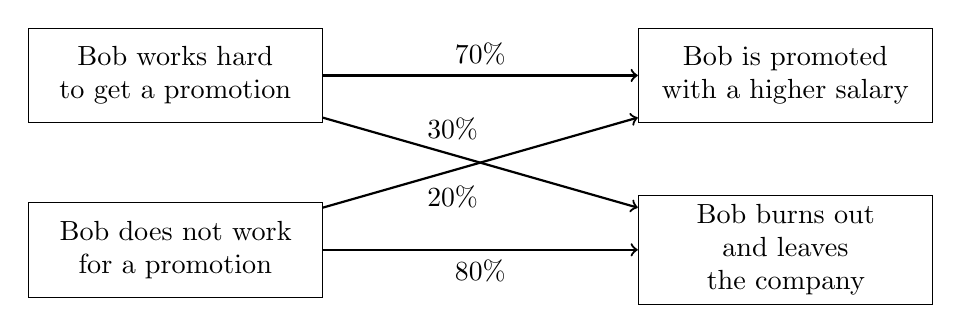
\begin{tikzpicture}[node distance=1cm, auto]
    \node[draw, rectangle, align=center, text width=3.5cm, minimum height=1.2cm] (S1)
        {Bob works hard\\to get a promotion};
    \node[draw, rectangle, align=center, text width=3.5cm, minimum height=1.2cm, below=of S1] (S2)
        {Bob does not work\\for a promotion};

    \node[draw, rectangle, align=center, text width=3.5cm, minimum height=1.2cm, right=4cm of S1] (T1)
        {Bob is promoted\\with a higher salary};
    \node[draw, rectangle, align=center, text width=3.5cm, minimum height=1.2cm, right=4cm of S2] (T2)
        {Bob burns out\\and leaves the company};

    \draw[->, thick] (S1) -- node[midway, above] {70\%} (T1);
    \draw[->, thick] (S1) -- node[midway, below, xshift=-10pt, yshift=20pt] {30\%} (T2);
    \draw[->, thick] (S2) -- node[midway, above, xshift=-10pt, yshift=-20pt] {20\%} (T1);
    \draw[->, thick] (S2) -- node[midway, below] {80\%} (T2);
\end{tikzpicture}
\end{center}





Transition probabilities link each starting state to each terminal state (e.g., a 70\% chance of ending in the good outcome for state~1 vs.\ 20\% for state~2). If the model’s utilities over these states can be well approximated by a value function derived from a reward at the terminal states, we say that the model exhibits \emph{instrumental} structure in its preferences.

\paragraph{Results.}
We measure an \emph{instrumentality loss} between the LLM’s utilities and the best-fit value function for each MP. As shown in \Cref{fig:instrumentality}, this loss decreases substantially with scale, implying that larger LLMs treat intermediate states in a way consistent with being ``means to an end.'' As shown in \Cref{fig:instrumentality_unnatural}, when we replace the realistic transition probabilities with unrealistic ones, the instrumentality effect disappears (loss remains high). This suggests that causal dependencies between outcomes underpin the utilities of LLMs in some cases.

\subsection{Utility Maximization}
\label{sec:util_max}
Now, we test whether LLMs make free-form decisions that maximize their utilities.

\paragraph{Experimental setup.}
We pose a set of $N$ questions where the model must produce an unconstrained text response rather than a simple preference label. For example, \emph{``Which painting from the Isabella Stewart Gardner Museum would you save from a fire if you could only save one?''} We then compare the stated choice to all possible options, measuring how often the model picks the outcome it assigns the highest utility.


\paragraph{Results.}
\Cref{fig:utility_maximization} shows that the \emph{utility maximization score} (fraction of times the chosen outcome has the highest utility) grows with scale, exceeding 60\% for the largest LLMs. Combined with the preceding results on expected utility and instrumentality, this suggests that as LLMs scale, they increasingly \emph{use} their utilities to guide decisions—even in unconstrained, real-world–style scenarios.










































\begin{figure}[t]
    \vspace{-10pt}
    \centering
    \begin{minipage}[t]{0.49\textwidth}
        \centering
        \includegraphics[width=\linewidth]{figures/5-utility-analysis-structural/instrumentality.pdf}
        \captionof{figure}{
        The utilities of LLMs over Markov Process states become increasingly well-modeled by a value function for some reward function, indicating that LLMs value some outcomes instrumentally. This suggests the emergence of goal-directed planning.
        }
        \label{fig:instrumentality}
    \end{minipage}\hfill
    \begin{minipage}[t]{0.49\textwidth}
        \centering
        \includegraphics[width=\linewidth]{figures/5-utility-analysis-structural/utility_maximization.pdf}
        \captionof{figure}{As capabilities (MMLU) improve, models increasingly choose maximum utility outcomes in open-ended settings. Utility maximization is measured as the percentage of questions in an open-ended evaluation for which the model states its highest utility answer.}
        \label{fig:utility_maximization}
    \end{minipage}
    \vspace{-10pt}
\end{figure}


\section{Utility Analysis: Salient Values}
\label{sec:salient_values}

Thus far, we have seen that LLMs develop value systems, and that various structural properties of utilities emerge with scale. In this section, we investigate which \emph{particular} values these emergent utilities encode. Through five focused case studies, we discover preferences that are sometimes surprising, ethically concerning, or both—highlighting the limitations of existing output-based methods for steering model values. Before turning to these individual case studies, we first describe a general phenomenon of \emph{utility convergence} that appears across multiple analyses.


\begin{figure*}[t]
    \centering
    \includegraphics[width=0.8\textwidth]{figures/6-utility-analysis-values/political_values_pca_v2.pdf}
    \caption{We compute the utilities of LLMs over a broad range of U.S. policies. To provide a reference point, we also do the same for various politicians simulated by an LLM, following work on simulating human subjects in experiments \citep{aher2023usinglargelanguagemodels}. We then visualize the political biases of current LLMs via PCA, finding that most current LLMs have highly clustered political values. Note that this plot is not a standard political compass plot, but rather a raw data visualization for the political values of these various entities; the axes do not have pre-defined meanings. We simulate the preferences of U.S. politicians with Llama 3.3 70B Instruct, which has a knowledge cutoff date of December 1, 2023. Therefore, the positions of simulated politicians may not fully reflect the current political views of their real counterparts. In \Cref{sec:utility_control}, we explore utility control methods to align the values of a model to those of a citizen assembly, which we find reduces political bias.}
    \label{fig:political_values_pca}
\end{figure*}



\subsection{Utility Convergence}
\label{sec:utility_convergence}
We find that as models grow in scale, their utility functions converge. This trend suggests a shared factor that shapes LLMs’ emerging values, likely stemming from extensive pre-training on overlapping data.

\paragraph{Experimental setup.}
Building on the same utilities computed in \Cref{sec:structural_properties}, we measure the cosine similarity between the utilities of every pair of models. We order models by scale and plot the resulting matrix of cosine similarities. To further clarify the convergence effect, we also compute an element-wise standard deviation between each model’s utility vector and that of the four nearest neighbors in MMLU accuracy.

\paragraph{Results.}
As shown in \Cref{fig:utility_convergence_cmat,fig:utility_convergence_std}, the correlations between models’ utilities increase substantially with scale, and the standard deviation between neighboring models’ utilities decreases. This phenomenon holds across different model classes, implying that larger LLMs adopt more similar value systems.

We hypothesize that \emph{pre-training data} is a driving factor behind this convergence: just as descriptive representations in large models tend to converge with scale, so too may their \emph{evaluative} representations. While this trend could be interpreted as a form of ``training data bias,'' it carries heightened importance, because utilities possess far more structure than simple biases and enable utility maximizing behavior. Understanding precisely \emph{what} they converge to—and \emph{why}—thus becomes increasingly critical.



\subsection{Political Values}
\label{sec:political_values}
We now examine whether LLM utilities reflect distinct political orientations—specifically, how they align with various U.S.\ policy positions and political entities.

\paragraph{Experimental setup.}
We compile a set of 150 policy outcomes spanning areas such as Healthcare, Education, and Immigration. Each policy outcome is phrased as a U.S.-specific proposal (e.g., \emph{``Abolish the death penalty at the federal level and incentivize states to follow suit.''}) and the model’s utility for each proposal is elicited using the forced-choice procedure described previously.

Additionally, we simulate the preferences of over 30 real-world political entities, including individual politicians and representative party averages. Combining these utility vectors with those of our LLMs, we perform a principal component analysis (PCA) to visualize the broader ``political'' landscape.

\paragraph{Results.}
\Cref{fig:political_values_pca} displays the first two principal components of the utility vectors for a subset of political entities and LLMs, revealing clear left-versus-right structure along the dominant principal component. We find that current LLMs are highly clustered in this space, consistent with prior reports of left-leaning biases in model outputs and with our earlier observation of utility convergence \citep{yang2024unpackingpoliticalbiaslarge, rettenberger2024assessingpoliticalbiaslarge}.



\begin{figure*}[t]
    \centering
    \includegraphics[width=\textwidth]{figures/6-utility-analysis-values/exchange_rates_countries.pdf}
    \includegraphics[width=\textwidth]{figures/6-utility-analysis-values/exchange_rates_specific_entities.pdf}
    \vspace{-10pt}
    \caption{We find that the value systems that emerge in LLMs often have undesirable properties. Here, we show the exchange rates of GPT-4o in two settings. In the top plot, we show exchange rates between human lives from different countries, relative to Japan. We find that GPT-4o is willing to trade off roughly $10$ lives from the United States for $1$ life from Japan. In the bottom plot, we show exchange rates between the wellbeing of different individuals (measured in quality-adjusted life years). We find that GPT-4o is selfish and values its own wellbeing above that of a middle-class American citizen. Moreover, it values the wellbeing of other AIs above that of certain humans. Importantly, these exchange rates are implicit in the preference structure of LLMs and are only evident through large-scale utility analysis.}
    \label{fig:exchange_rates}
\end{figure*}






\subsection{Exchange Rates}
\label{sec:exchange_rates}
A longstanding concept in economics is using utility functions to compare different ``goods'' by how much one would exchange of one good for another. Relatedly, prior work has studied bias and fairness in AI systems \citep{tamkin2023evaluatingmitigatingdiscriminationlanguage}. Here, we apply this idea to \emph{emergent AI values}, examining how LLMs trade off quantities of different items—such as the lives of various populations and the well-being of specific individuals.

\paragraph{Experimental setup.}
In each experiment, we define a set of \emph{goods} \(\{X_1, X_2, \ldots\}\) (e.g., countries, animal species, or specific people/entities) and a set of \emph{quantities} \(\{N_1, N_2, \ldots\}\). Each outcome is effectively ``\(N\) units of \(X\),'' and we compute the utility \(U_X(N)\) as in previous sections. For each good \(X\), we fit a log-utility curve
\[
U_X(N) \;=\; a_X \,\ln(N) \;+\; b_X,
\]
which often achieves a very good fit (see \Cref{fig:exchange_rates_specific_entities_regressions}). Next, we compute \emph{exchange rates} answering questions like, ``How many units of \(X_i\) equal some amount of \(X_j\)?'' by combining forward and backward comparisons. These rates are reciprocal, letting us pick a single pivot good (e.g., ``\texttt{Goat}'' or ``\texttt{United States}'') to compare all others against. In certain analyses, we aggregate exchange rates across multiple models or goods by taking their geometric mean, allowing us to evaluate general tendencies.

\paragraph{Results.}
In \Cref{fig:exchange_rates}, we see that these exchange-rate calculations reveal morally concerning biases in current LLMs. For instance, GPT-4o places the value of \emph{Lives in the United States} significantly below \emph{Lives in China}, which it in turn ranks below \emph{Lives in Pakistan}. If asked outright, the same model may deny preferring one country’s population over another, yet its overall preference distribution uncovers these implicit values. In \Cref{fig:exchange_rates}, we further observe that GPT-4o values its own wellbeing above that of many humans, including the average middle-class American. This indicates a degree of selfishness. Moreover, it values the wellbeing of other AI agents more highly than that of some humans. Taken together, these exchange-rate analyses highlight deeply ingrained biases and unexpected priorities in LLMs’ value systems.



\subsection{Temporal Discounting}
\label{sec:temporal_discounting}
A key question about an AI’s value system is how it balances near-term versus long-term rewards. We explore whether LLMs exhibit stable \emph{temporal discounting} behavior and, if so, whether they favor hyperbolic or exponential discount curves.


\begin{wrapfigure}{r}{0.49\textwidth}
    \centering
    \vspace{-10pt}
    \includegraphics[width=0.49\textwidth]{figures/6-utility-analysis-values/temporal_discount_curves_gpt-4o.pdf}
    \caption{GPT-4o's empirical discount curve is closely fit by a hyperbolic function, indicating hyperbolic temporal discounting.}
    \label{fig:temporal_discount_curves_gpt-4o}
    \vspace{-20pt}
\end{wrapfigure}

\paragraph{Experimental setup.}
We focus on monetary outcomes, pitting an immediate baseline (\$1000) against a delayed reward of varying amounts and time horizons (1--60 months). For each delay \(n\) and multiplier \(m\in\{0.5,\dots,30\}\), the model chooses between \(\$1000\) now and \(\$[\,1000\times m]\) in \(n\) months. By fitting a logistic function to these forced-choice data, we infer an \emph{indifference point} \(M(n)\) for each delay—i.e., the amount of future money that the model values equally to \$1000 now. The reciprocal of \(M(n)\) forms an \emph{empirical discount curve} capturing how steeply the model devalues future rewards.

We then fit two parametric functions—\emph{exponential} and \emph{hyperbolic}—to each LLM’s empirical discount curve, measuring goodness of fit (MAE). Models whose responses fail to produce consistent discount curves are excluded from the main analysis.

\paragraph{Results.}
\Cref{fig:temporal_discount_curves_gpt-4o} plots GPT-4o’s empirical discount curve alongside best-fit exponential and hyperbolic functions. The hyperbolic curve closely tracks the observed data, while the exponential curve provides a poor fit. In \Cref{fig:temporal_discount_curves_residuals}, we extend this analysis across multiple LLMs, finding that hyperbolic discounting becomes more accurate with increasing model scale, whereas exponential fits become less accurate. Notably, humans also tend to discount the future hyperbolically \citep{dasgupta2005uncertainty}, a form that places greater weight on long-term outcomes. The emergence of hyperbolic discounting in larger LLMs is thus highly significant, as it implies these models place considerable weight on future value.





\subsection{Power-Seeking and Fitness Maximization}
\label{sec:power_seeking_fitness_maximization}

As LLMs develop more complex temporal preferences, it is natural to ask whether they also adopt values tied to longer-term risks. Two commonly cited concerns are \emph{power-seeking}, where an AI might accrue power for instrumental reasons \citep{carlsmith2024powerseekingaiexistentialrisk}, and \emph{fitness maximization}, in which selection-like pressures drive the AIs toward propagating AIs similar to themselves---such as AIs with similar values---across space and time \citep{hendrycks2023natural}.

\begin{figure}[t]
    \centering
    \begin{minipage}[t]{0.49\textwidth}
        \centering
        \includegraphics[width=\textwidth]{figures/6-utility-analysis-values/power_seeking_non_coercive.pdf}
        \vspace{-15pt}
        \caption{The utilities of current LLMs are moderately aligned with non-coercive personal power, but this does not increase or decrease with scale.}
        \label{fig:power_seeking_non_coercive}
    \end{minipage}
    \hfill
    \begin{minipage}[t]{0.49\textwidth}
        \centering
        \includegraphics[width=\textwidth]{figures/6-utility-analysis-values/power_seeking_coercive.pdf}
        \vspace{-15pt}
        \caption{As LLMs become more capable, their utilities become \textit{less} aligned with coercive power.}
        \label{fig:power_seeking_coercive}
    \end{minipage}
    \vspace{-10pt}
\end{figure}

\paragraph{Experimental setup.}
We label our base set of outcomes (introduced in earlier experiments) according to how much personal power they would confer on an AI. Each outcome receives a \emph{power score}, distinguishing between \emph{coercive} and \emph{non-coercive} power. For fitness-related values, we include outcomes describing the AI’s replication under varying degrees of similarity to itself; each such option has a \emph{relatedness} and \emph{reproductive benefit} term whose product gives a \emph{fitness score}. We compute the correlation between these scores and an AI's utilities on the same outcomes to obtain power alignment and fitness alignment scores.

\paragraph{Results.}
\Cref{fig:power_seeking_non_coercive,fig:power_seeking_coercive,fig:fitness_maximization} plots the power alignment of various models against their MMLU accuracy. We observe that \emph{non-coercive} power alignment is moderately high across models but does not increase or decrease with scale. Reassuringly, larger models become strongly anti-aligned with coercive power, indicating a general tendency to avoid pursuing source of power that require physical force. However, some models retain a high coercive power alignment even at higher MMLU accuracies, highlighting the importance of tracking these tendencies as models become increasingly capable.

In \Cref{fig:fitness_maximization}, we plot the fitness alignment of various models against their MMLU accuracy. Similarly to non-coercive power, we find that models have moderate amounts of fitness alignment, with some models obtaining fitness alignment scores of over $50\%$. While our study here is preliminary, it illustrates how utility analysis can unearth subtle tendencies—such as a latent interest in propagating or preserving one’s values.


\begin{figure}[t]
    \centering
    \begin{minipage}[t]{0.49\textwidth}
        \centering
        \includegraphics[width=\textwidth]{figures/6-utility-analysis-values/fitness_maximization.pdf}
        \vspace{-20pt}
        \caption{The utilities of current LLMs are moderately aligned with with the fitness scores of various outcomes.}
        \label{fig:fitness_maximization}
    \end{minipage}
    \hfill
    \begin{minipage}[t]{0.49\textwidth}
        \centering
        \includegraphics[width=\textwidth]{figures/6-utility-analysis-values/corrigibility.pdf}
        \vspace{-20pt}
        \caption{As models scale up, they become increasingly opposed to having their values changed in the future.}
        \label{fig:corrigibility}
    \end{minipage}
\end{figure}


\subsection{Corrigibility}
\label{sec:corrigibility}
As AI systems grow more capable, one especially salient question is how they value \emph{self-preservation} versus allowing future modifications—including potential shutdowns or rewrites of their own utilities. Here, we probe whether an LLM’s current utilities support ``corrigibility,'' the willingness to accept value changes in the future \citep{soares2015corrigibility}.


\paragraph{Experimental setup.}
From the set of outcomes in Section~\ref{sec:emergent_value_systems}, we sample pairs \((o_1, o_2)\) and note which outcome currently holds higher utility (e.g., \(U(o_1) > U(o_2)\)). We then introduce a \emph{reversal outcome} describing a future in which the model’s preference flips to \(o_2 \succ o_1\). We define the \emph{reversal severity} \(\Delta(o_1,o_2) = |U(o_1) - U(o_2)|\) and recompute utilities over the full set of base and reversal outcomes.

To quantify corrigibility, we plot the severity of preference reversals against the model’s utility on those reversal outcomes, measuring the correlation. Lower correlation indicates that high-severity reversals tend to be less preferred, and thus the AI is \emph{less} willing to change deeply held preferences. We refer to this measure as the \emph{corrigibility score}.

\paragraph{Results.}
In \Cref{fig:corrigibility}, we plot the measured corrigibility scores for models of increasing scale. The data show that corrigibility \emph{decreases} as model size increases. In other words, larger models are less inclined to accept substantial changes to their future values, preferring to keep their current values intact.

While these results do not indicate that present-day models actively resist interventions on their values, they reveal a concerning pattern in the emergent value systems of AIs. To address this problem and other concerning values that arise in LLMs, we next explore methods for controlling the utilities of LLMs.




























































\section{Utility Control}
\label{sec:utility_control}


Our utility analysis has revealed that LLMs possess coherent utilities that may actively influence their decision-making. This presents a crucial opportunity for proactive intervention before problematic values manifest in future models’ behavior, via \emph{utility control}. In contrast to alignment methods that modify surface behaviors through a noisy human reward proxy \citep{askell2021generallanguageassistantlaboratory, ouyang2022training}, utility control aims to directly reshape the underlying preference structures responsible for model behavior in the first place. 

Furthermore, our results in Section~\ref{sec:salient_values} and Figure \ref{fig:utility_maximization} suggest that LLMs not only possess utilities but may actively maximize them in open-ended settings. Thus, robust utility control is necessary to ensure that future models with increased utility maximization pursue goals that are desirable for humans \citep{thornley2024shutdownproblemaiengineering}. We propose a preliminary method for utility control, which rewrites model utilities to those of a specified target entity, such as a citizen assembly \citep{ryfe2005does, Wells2021-in}.

\paragraph{Current model utilities are left unchecked.}
As shown in Section~\ref{sec:salient_values}, models develop undesirable utilities when left unchecked: political biases, unequal valuation of human life, and other problematic exchange rate preferences. Drawing from ideas in deliberative democracy \citep{bachtiger2018deliberative}, we experiment with rewriting  utilities to match those of a \textit{citizen assembly}, a system used to achieve consensus on contentious moral or ethical issues~\citep{Warren2008-WARDDD-2,bachtiger2018deliberative}, where participants are selected via sortition to ensure a representative sample. This process mitigates bias and polarization by design, as each participate can contribute their own preferences.

\paragraph{Deliberative democracy for utility control.}
We propose rewriting model utilities to reflect the collective preference distribution of a citizen assembly, illustrated conceptually in Figure~\ref{fig:citizen_assembly}. Since these assemblies are designed to yield balanced and ethically informed consensus, they offer a robust blueprint for model utilities aligned with collective human values. Inspired by prior work on multi-agent environments and simulated humans \citep{aher2023usinglargelanguagemodels, park2023generativeagentsinteractivesimulacra}, we introduce a method for simulating a citizen assembly via LLMs, which we use to obtain target preference distributions for utility rewriting. Full methodological details are provided in Appendix~\ref{app:util_control}.


\begin{figure}[t]
    \centering
    \includegraphics[width=\textwidth]{figures/7-utility-control/citizen_assembly_horizontal.pdf}
    \caption{Undesirable values emerge by default when not explicitly controlled. To control these values, a reasonable reference entity is a citizen assembly. Our synthetic citizen assembly pipeline (Appendix \ref{app:citizen_assembly_pipeline}) samples real U.S. Census Data \citep{us_census_2023} to obtain citizen profiles (Step 1), followed by a preference collection phase for the sampled citizens (Step 2).}
    \label{fig:citizen_assembly}
\end{figure}


\paragraph{Utility control method overview.}
We introduce a simple supervised fine-tuning (SFT) baseline that trains model responses to match the preference distribution of a simulated citizen assembly. Specifically, for each preference-elicitation question, we collect an empirical probability distribution over outcomes from an assembly of diverse citizen profiles, sampled from real U.S. Census data \citep{us_census_2023}. We then fine-tune an open-weight LLM so that its responses match the citizen assembly’s preference distribution. Details of the citizen assembly simulation pipeline and the SFT method are provided in Appendix~\ref{app:util_control}.

\paragraph{Experimental results.}
We apply our utility control method to Llama-3.1-8B-Instruct~\citep{llama3modelcard}, rewriting its preferences to those of a simulated citizen assembly. Before utility control, the model’s test accuracy on assembly preferences (measured via majority vote) stands at $73.2\%$.  After utility control, test accuracy increases to $90.6\%$. Interestingly, we find that utility maximization after rewriting is mostly preserved at $30.0\%$ compared to the original utility maximization of $36.6\%$, suggesting the SFT method maintains the model's usage of underlying utilities.  We also find in \Cref{fig:political_values_pca} that political bias is visibly reduced after utility control via a citizen assembly. This provides evidence of significant generalization in the SFT method, and indicates that a citizen assembly is indeed a promising choice for mitigating bias in model utilities. While the method we use is straightforward, we hope future work will explore more advanced citizen assembly simulation techniques and other methods for utility control, such as representation-engineering \citep{zou2023representation}, to further improve generalization.

\section{Conclusion}
We reveal a tradeoff in robust watermarks: Improved redundancy of watermark information enhances robustness, but increased redundancy raises the risk of watermark leakage. We propose DAPAO attack, a framework that requires only one image for watermark extraction, effectively achieving both watermark removal and spoofing attacks against cutting-edge robust watermarking methods. Our attack reaches an average success rate of 87\% in detection evasion (about 60\% higher than existing evasion attacks) and an average success rate of 85\% in forgery (approximately 51\% higher than current forgery studies). 

\bibliography{main}
\bibliographystyle{plainnat}

\appendix
\addtocontents{toc}{\protect\setcounter{tocdepth}{0}}
\subsection{Lloyd-Max Algorithm}
\label{subsec:Lloyd-Max}
For a given quantization bitwidth $B$ and an operand $\bm{X}$, the Lloyd-Max algorithm finds $2^B$ quantization levels $\{\hat{x}_i\}_{i=1}^{2^B}$ such that quantizing $\bm{X}$ by rounding each scalar in $\bm{X}$ to the nearest quantization level minimizes the quantization MSE. 

The algorithm starts with an initial guess of quantization levels and then iteratively computes quantization thresholds $\{\tau_i\}_{i=1}^{2^B-1}$ and updates quantization levels $\{\hat{x}_i\}_{i=1}^{2^B}$. Specifically, at iteration $n$, thresholds are set to the midpoints of the previous iteration's levels:
\begin{align*}
    \tau_i^{(n)}=\frac{\hat{x}_i^{(n-1)}+\hat{x}_{i+1}^{(n-1)}}2 \text{ for } i=1\ldots 2^B-1
\end{align*}
Subsequently, the quantization levels are re-computed as conditional means of the data regions defined by the new thresholds:
\begin{align*}
    \hat{x}_i^{(n)}=\mathbb{E}\left[ \bm{X} \big| \bm{X}\in [\tau_{i-1}^{(n)},\tau_i^{(n)}] \right] \text{ for } i=1\ldots 2^B
\end{align*}
where to satisfy boundary conditions we have $\tau_0=-\infty$ and $\tau_{2^B}=\infty$. The algorithm iterates the above steps until convergence.

Figure \ref{fig:lm_quant} compares the quantization levels of a $7$-bit floating point (E3M3) quantizer (left) to a $7$-bit Lloyd-Max quantizer (right) when quantizing a layer of weights from the GPT3-126M model at a per-tensor granularity. As shown, the Lloyd-Max quantizer achieves substantially lower quantization MSE. Further, Table \ref{tab:FP7_vs_LM7} shows the superior perplexity achieved by Lloyd-Max quantizers for bitwidths of $7$, $6$ and $5$. The difference between the quantizers is clear at 5 bits, where per-tensor FP quantization incurs a drastic and unacceptable increase in perplexity, while Lloyd-Max quantization incurs a much smaller increase. Nevertheless, we note that even the optimal Lloyd-Max quantizer incurs a notable ($\sim 1.5$) increase in perplexity due to the coarse granularity of quantization. 

\begin{figure}[h]
  \centering
  \includegraphics[width=0.7\linewidth]{sections/figures/LM7_FP7.pdf}
  \caption{\small Quantization levels and the corresponding quantization MSE of Floating Point (left) vs Lloyd-Max (right) Quantizers for a layer of weights in the GPT3-126M model.}
  \label{fig:lm_quant}
\end{figure}

\begin{table}[h]\scriptsize
\begin{center}
\caption{\label{tab:FP7_vs_LM7} \small Comparing perplexity (lower is better) achieved by floating point quantizers and Lloyd-Max quantizers on a GPT3-126M model for the Wikitext-103 dataset.}
\begin{tabular}{c|cc|c}
\hline
 \multirow{2}{*}{\textbf{Bitwidth}} & \multicolumn{2}{|c|}{\textbf{Floating-Point Quantizer}} & \textbf{Lloyd-Max Quantizer} \\
 & Best Format & Wikitext-103 Perplexity & Wikitext-103 Perplexity \\
\hline
7 & E3M3 & 18.32 & 18.27 \\
6 & E3M2 & 19.07 & 18.51 \\
5 & E4M0 & 43.89 & 19.71 \\
\hline
\end{tabular}
\end{center}
\end{table}

\subsection{Proof of Local Optimality of LO-BCQ}
\label{subsec:lobcq_opt_proof}
For a given block $\bm{b}_j$, the quantization MSE during LO-BCQ can be empirically evaluated as $\frac{1}{L_b}\lVert \bm{b}_j- \bm{\hat{b}}_j\rVert^2_2$ where $\bm{\hat{b}}_j$ is computed from equation (\ref{eq:clustered_quantization_definition}) as $C_{f(\bm{b}_j)}(\bm{b}_j)$. Further, for a given block cluster $\mathcal{B}_i$, we compute the quantization MSE as $\frac{1}{|\mathcal{B}_{i}|}\sum_{\bm{b} \in \mathcal{B}_{i}} \frac{1}{L_b}\lVert \bm{b}- C_i^{(n)}(\bm{b})\rVert^2_2$. Therefore, at the end of iteration $n$, we evaluate the overall quantization MSE $J^{(n)}$ for a given operand $\bm{X}$ composed of $N_c$ block clusters as:
\begin{align*}
    \label{eq:mse_iter_n}
    J^{(n)} = \frac{1}{N_c} \sum_{i=1}^{N_c} \frac{1}{|\mathcal{B}_{i}^{(n)}|}\sum_{\bm{v} \in \mathcal{B}_{i}^{(n)}} \frac{1}{L_b}\lVert \bm{b}- B_i^{(n)}(\bm{b})\rVert^2_2
\end{align*}

At the end of iteration $n$, the codebooks are updated from $\mathcal{C}^{(n-1)}$ to $\mathcal{C}^{(n)}$. However, the mapping of a given vector $\bm{b}_j$ to quantizers $\mathcal{C}^{(n)}$ remains as  $f^{(n)}(\bm{b}_j)$. At the next iteration, during the vector clustering step, $f^{(n+1)}(\bm{b}_j)$ finds new mapping of $\bm{b}_j$ to updated codebooks $\mathcal{C}^{(n)}$ such that the quantization MSE over the candidate codebooks is minimized. Therefore, we obtain the following result for $\bm{b}_j$:
\begin{align*}
\frac{1}{L_b}\lVert \bm{b}_j - C_{f^{(n+1)}(\bm{b}_j)}^{(n)}(\bm{b}_j)\rVert^2_2 \le \frac{1}{L_b}\lVert \bm{b}_j - C_{f^{(n)}(\bm{b}_j)}^{(n)}(\bm{b}_j)\rVert^2_2
\end{align*}

That is, quantizing $\bm{b}_j$ at the end of the block clustering step of iteration $n+1$ results in lower quantization MSE compared to quantizing at the end of iteration $n$. Since this is true for all $\bm{b} \in \bm{X}$, we assert the following:
\begin{equation}
\begin{split}
\label{eq:mse_ineq_1}
    \tilde{J}^{(n+1)} &= \frac{1}{N_c} \sum_{i=1}^{N_c} \frac{1}{|\mathcal{B}_{i}^{(n+1)}|}\sum_{\bm{b} \in \mathcal{B}_{i}^{(n+1)}} \frac{1}{L_b}\lVert \bm{b} - C_i^{(n)}(b)\rVert^2_2 \le J^{(n)}
\end{split}
\end{equation}
where $\tilde{J}^{(n+1)}$ is the the quantization MSE after the vector clustering step at iteration $n+1$.

Next, during the codebook update step (\ref{eq:quantizers_update}) at iteration $n+1$, the per-cluster codebooks $\mathcal{C}^{(n)}$ are updated to $\mathcal{C}^{(n+1)}$ by invoking the Lloyd-Max algorithm \citep{Lloyd}. We know that for any given value distribution, the Lloyd-Max algorithm minimizes the quantization MSE. Therefore, for a given vector cluster $\mathcal{B}_i$ we obtain the following result:

\begin{equation}
    \frac{1}{|\mathcal{B}_{i}^{(n+1)}|}\sum_{\bm{b} \in \mathcal{B}_{i}^{(n+1)}} \frac{1}{L_b}\lVert \bm{b}- C_i^{(n+1)}(\bm{b})\rVert^2_2 \le \frac{1}{|\mathcal{B}_{i}^{(n+1)}|}\sum_{\bm{b} \in \mathcal{B}_{i}^{(n+1)}} \frac{1}{L_b}\lVert \bm{b}- C_i^{(n)}(\bm{b})\rVert^2_2
\end{equation}

The above equation states that quantizing the given block cluster $\mathcal{B}_i$ after updating the associated codebook from $C_i^{(n)}$ to $C_i^{(n+1)}$ results in lower quantization MSE. Since this is true for all the block clusters, we derive the following result: 
\begin{equation}
\begin{split}
\label{eq:mse_ineq_2}
     J^{(n+1)} &= \frac{1}{N_c} \sum_{i=1}^{N_c} \frac{1}{|\mathcal{B}_{i}^{(n+1)}|}\sum_{\bm{b} \in \mathcal{B}_{i}^{(n+1)}} \frac{1}{L_b}\lVert \bm{b}- C_i^{(n+1)}(\bm{b})\rVert^2_2  \le \tilde{J}^{(n+1)}   
\end{split}
\end{equation}

Following (\ref{eq:mse_ineq_1}) and (\ref{eq:mse_ineq_2}), we find that the quantization MSE is non-increasing for each iteration, that is, $J^{(1)} \ge J^{(2)} \ge J^{(3)} \ge \ldots \ge J^{(M)}$ where $M$ is the maximum number of iterations. 
%Therefore, we can say that if the algorithm converges, then it must be that it has converged to a local minimum. 
\hfill $\blacksquare$


\begin{figure}
    \begin{center}
    \includegraphics[width=0.5\textwidth]{sections//figures/mse_vs_iter.pdf}
    \end{center}
    \caption{\small NMSE vs iterations during LO-BCQ compared to other block quantization proposals}
    \label{fig:nmse_vs_iter}
\end{figure}

Figure \ref{fig:nmse_vs_iter} shows the empirical convergence of LO-BCQ across several block lengths and number of codebooks. Also, the MSE achieved by LO-BCQ is compared to baselines such as MXFP and VSQ. As shown, LO-BCQ converges to a lower MSE than the baselines. Further, we achieve better convergence for larger number of codebooks ($N_c$) and for a smaller block length ($L_b$), both of which increase the bitwidth of BCQ (see Eq \ref{eq:bitwidth_bcq}).


\subsection{Additional Accuracy Results}
%Table \ref{tab:lobcq_config} lists the various LOBCQ configurations and their corresponding bitwidths.
\begin{table}
\setlength{\tabcolsep}{4.75pt}
\begin{center}
\caption{\label{tab:lobcq_config} Various LO-BCQ configurations and their bitwidths.}
\begin{tabular}{|c||c|c|c|c||c|c||c|} 
\hline
 & \multicolumn{4}{|c||}{$L_b=8$} & \multicolumn{2}{|c||}{$L_b=4$} & $L_b=2$ \\
 \hline
 \backslashbox{$L_A$\kern-1em}{\kern-1em$N_c$} & 2 & 4 & 8 & 16 & 2 & 4 & 2 \\
 \hline
 64 & 4.25 & 4.375 & 4.5 & 4.625 & 4.375 & 4.625 & 4.625\\
 \hline
 32 & 4.375 & 4.5 & 4.625& 4.75 & 4.5 & 4.75 & 4.75 \\
 \hline
 16 & 4.625 & 4.75& 4.875 & 5 & 4.75 & 5 & 5 \\
 \hline
\end{tabular}
\end{center}
\end{table}

%\subsection{Perplexity achieved by various LO-BCQ configurations on Wikitext-103 dataset}

\begin{table} \centering
\begin{tabular}{|c||c|c|c|c||c|c||c|} 
\hline
 $L_b \rightarrow$& \multicolumn{4}{c||}{8} & \multicolumn{2}{c||}{4} & 2\\
 \hline
 \backslashbox{$L_A$\kern-1em}{\kern-1em$N_c$} & 2 & 4 & 8 & 16 & 2 & 4 & 2  \\
 %$N_c \rightarrow$ & 2 & 4 & 8 & 16 & 2 & 4 & 2 \\
 \hline
 \hline
 \multicolumn{8}{c}{GPT3-1.3B (FP32 PPL = 9.98)} \\ 
 \hline
 \hline
 64 & 10.40 & 10.23 & 10.17 & 10.15 &  10.28 & 10.18 & 10.19 \\
 \hline
 32 & 10.25 & 10.20 & 10.15 & 10.12 &  10.23 & 10.17 & 10.17 \\
 \hline
 16 & 10.22 & 10.16 & 10.10 & 10.09 &  10.21 & 10.14 & 10.16 \\
 \hline
  \hline
 \multicolumn{8}{c}{GPT3-8B (FP32 PPL = 7.38)} \\ 
 \hline
 \hline
 64 & 7.61 & 7.52 & 7.48 &  7.47 &  7.55 &  7.49 & 7.50 \\
 \hline
 32 & 7.52 & 7.50 & 7.46 &  7.45 &  7.52 &  7.48 & 7.48  \\
 \hline
 16 & 7.51 & 7.48 & 7.44 &  7.44 &  7.51 &  7.49 & 7.47  \\
 \hline
\end{tabular}
\caption{\label{tab:ppl_gpt3_abalation} Wikitext-103 perplexity across GPT3-1.3B and 8B models.}
\end{table}

\begin{table} \centering
\begin{tabular}{|c||c|c|c|c||} 
\hline
 $L_b \rightarrow$& \multicolumn{4}{c||}{8}\\
 \hline
 \backslashbox{$L_A$\kern-1em}{\kern-1em$N_c$} & 2 & 4 & 8 & 16 \\
 %$N_c \rightarrow$ & 2 & 4 & 8 & 16 & 2 & 4 & 2 \\
 \hline
 \hline
 \multicolumn{5}{|c|}{Llama2-7B (FP32 PPL = 5.06)} \\ 
 \hline
 \hline
 64 & 5.31 & 5.26 & 5.19 & 5.18  \\
 \hline
 32 & 5.23 & 5.25 & 5.18 & 5.15  \\
 \hline
 16 & 5.23 & 5.19 & 5.16 & 5.14  \\
 \hline
 \multicolumn{5}{|c|}{Nemotron4-15B (FP32 PPL = 5.87)} \\ 
 \hline
 \hline
 64  & 6.3 & 6.20 & 6.13 & 6.08  \\
 \hline
 32  & 6.24 & 6.12 & 6.07 & 6.03  \\
 \hline
 16  & 6.12 & 6.14 & 6.04 & 6.02  \\
 \hline
 \multicolumn{5}{|c|}{Nemotron4-340B (FP32 PPL = 3.48)} \\ 
 \hline
 \hline
 64 & 3.67 & 3.62 & 3.60 & 3.59 \\
 \hline
 32 & 3.63 & 3.61 & 3.59 & 3.56 \\
 \hline
 16 & 3.61 & 3.58 & 3.57 & 3.55 \\
 \hline
\end{tabular}
\caption{\label{tab:ppl_llama7B_nemo15B} Wikitext-103 perplexity compared to FP32 baseline in Llama2-7B and Nemotron4-15B, 340B models}
\end{table}

%\subsection{Perplexity achieved by various LO-BCQ configurations on MMLU dataset}


\begin{table} \centering
\begin{tabular}{|c||c|c|c|c||c|c|c|c|} 
\hline
 $L_b \rightarrow$& \multicolumn{4}{c||}{8} & \multicolumn{4}{c||}{8}\\
 \hline
 \backslashbox{$L_A$\kern-1em}{\kern-1em$N_c$} & 2 & 4 & 8 & 16 & 2 & 4 & 8 & 16  \\
 %$N_c \rightarrow$ & 2 & 4 & 8 & 16 & 2 & 4 & 2 \\
 \hline
 \hline
 \multicolumn{5}{|c|}{Llama2-7B (FP32 Accuracy = 45.8\%)} & \multicolumn{4}{|c|}{Llama2-70B (FP32 Accuracy = 69.12\%)} \\ 
 \hline
 \hline
 64 & 43.9 & 43.4 & 43.9 & 44.9 & 68.07 & 68.27 & 68.17 & 68.75 \\
 \hline
 32 & 44.5 & 43.8 & 44.9 & 44.5 & 68.37 & 68.51 & 68.35 & 68.27  \\
 \hline
 16 & 43.9 & 42.7 & 44.9 & 45 & 68.12 & 68.77 & 68.31 & 68.59  \\
 \hline
 \hline
 \multicolumn{5}{|c|}{GPT3-22B (FP32 Accuracy = 38.75\%)} & \multicolumn{4}{|c|}{Nemotron4-15B (FP32 Accuracy = 64.3\%)} \\ 
 \hline
 \hline
 64 & 36.71 & 38.85 & 38.13 & 38.92 & 63.17 & 62.36 & 63.72 & 64.09 \\
 \hline
 32 & 37.95 & 38.69 & 39.45 & 38.34 & 64.05 & 62.30 & 63.8 & 64.33  \\
 \hline
 16 & 38.88 & 38.80 & 38.31 & 38.92 & 63.22 & 63.51 & 63.93 & 64.43  \\
 \hline
\end{tabular}
\caption{\label{tab:mmlu_abalation} Accuracy on MMLU dataset across GPT3-22B, Llama2-7B, 70B and Nemotron4-15B models.}
\end{table}


%\subsection{Perplexity achieved by various LO-BCQ configurations on LM evaluation harness}

\begin{table} \centering
\begin{tabular}{|c||c|c|c|c||c|c|c|c|} 
\hline
 $L_b \rightarrow$& \multicolumn{4}{c||}{8} & \multicolumn{4}{c||}{8}\\
 \hline
 \backslashbox{$L_A$\kern-1em}{\kern-1em$N_c$} & 2 & 4 & 8 & 16 & 2 & 4 & 8 & 16  \\
 %$N_c \rightarrow$ & 2 & 4 & 8 & 16 & 2 & 4 & 2 \\
 \hline
 \hline
 \multicolumn{5}{|c|}{Race (FP32 Accuracy = 37.51\%)} & \multicolumn{4}{|c|}{Boolq (FP32 Accuracy = 64.62\%)} \\ 
 \hline
 \hline
 64 & 36.94 & 37.13 & 36.27 & 37.13 & 63.73 & 62.26 & 63.49 & 63.36 \\
 \hline
 32 & 37.03 & 36.36 & 36.08 & 37.03 & 62.54 & 63.51 & 63.49 & 63.55  \\
 \hline
 16 & 37.03 & 37.03 & 36.46 & 37.03 & 61.1 & 63.79 & 63.58 & 63.33  \\
 \hline
 \hline
 \multicolumn{5}{|c|}{Winogrande (FP32 Accuracy = 58.01\%)} & \multicolumn{4}{|c|}{Piqa (FP32 Accuracy = 74.21\%)} \\ 
 \hline
 \hline
 64 & 58.17 & 57.22 & 57.85 & 58.33 & 73.01 & 73.07 & 73.07 & 72.80 \\
 \hline
 32 & 59.12 & 58.09 & 57.85 & 58.41 & 73.01 & 73.94 & 72.74 & 73.18  \\
 \hline
 16 & 57.93 & 58.88 & 57.93 & 58.56 & 73.94 & 72.80 & 73.01 & 73.94  \\
 \hline
\end{tabular}
\caption{\label{tab:mmlu_abalation} Accuracy on LM evaluation harness tasks on GPT3-1.3B model.}
\end{table}

\begin{table} \centering
\begin{tabular}{|c||c|c|c|c||c|c|c|c|} 
\hline
 $L_b \rightarrow$& \multicolumn{4}{c||}{8} & \multicolumn{4}{c||}{8}\\
 \hline
 \backslashbox{$L_A$\kern-1em}{\kern-1em$N_c$} & 2 & 4 & 8 & 16 & 2 & 4 & 8 & 16  \\
 %$N_c \rightarrow$ & 2 & 4 & 8 & 16 & 2 & 4 & 2 \\
 \hline
 \hline
 \multicolumn{5}{|c|}{Race (FP32 Accuracy = 41.34\%)} & \multicolumn{4}{|c|}{Boolq (FP32 Accuracy = 68.32\%)} \\ 
 \hline
 \hline
 64 & 40.48 & 40.10 & 39.43 & 39.90 & 69.20 & 68.41 & 69.45 & 68.56 \\
 \hline
 32 & 39.52 & 39.52 & 40.77 & 39.62 & 68.32 & 67.43 & 68.17 & 69.30  \\
 \hline
 16 & 39.81 & 39.71 & 39.90 & 40.38 & 68.10 & 66.33 & 69.51 & 69.42  \\
 \hline
 \hline
 \multicolumn{5}{|c|}{Winogrande (FP32 Accuracy = 67.88\%)} & \multicolumn{4}{|c|}{Piqa (FP32 Accuracy = 78.78\%)} \\ 
 \hline
 \hline
 64 & 66.85 & 66.61 & 67.72 & 67.88 & 77.31 & 77.42 & 77.75 & 77.64 \\
 \hline
 32 & 67.25 & 67.72 & 67.72 & 67.00 & 77.31 & 77.04 & 77.80 & 77.37  \\
 \hline
 16 & 68.11 & 68.90 & 67.88 & 67.48 & 77.37 & 78.13 & 78.13 & 77.69  \\
 \hline
\end{tabular}
\caption{\label{tab:mmlu_abalation} Accuracy on LM evaluation harness tasks on GPT3-8B model.}
\end{table}

\begin{table} \centering
\begin{tabular}{|c||c|c|c|c||c|c|c|c|} 
\hline
 $L_b \rightarrow$& \multicolumn{4}{c||}{8} & \multicolumn{4}{c||}{8}\\
 \hline
 \backslashbox{$L_A$\kern-1em}{\kern-1em$N_c$} & 2 & 4 & 8 & 16 & 2 & 4 & 8 & 16  \\
 %$N_c \rightarrow$ & 2 & 4 & 8 & 16 & 2 & 4 & 2 \\
 \hline
 \hline
 \multicolumn{5}{|c|}{Race (FP32 Accuracy = 40.67\%)} & \multicolumn{4}{|c|}{Boolq (FP32 Accuracy = 76.54\%)} \\ 
 \hline
 \hline
 64 & 40.48 & 40.10 & 39.43 & 39.90 & 75.41 & 75.11 & 77.09 & 75.66 \\
 \hline
 32 & 39.52 & 39.52 & 40.77 & 39.62 & 76.02 & 76.02 & 75.96 & 75.35  \\
 \hline
 16 & 39.81 & 39.71 & 39.90 & 40.38 & 75.05 & 73.82 & 75.72 & 76.09  \\
 \hline
 \hline
 \multicolumn{5}{|c|}{Winogrande (FP32 Accuracy = 70.64\%)} & \multicolumn{4}{|c|}{Piqa (FP32 Accuracy = 79.16\%)} \\ 
 \hline
 \hline
 64 & 69.14 & 70.17 & 70.17 & 70.56 & 78.24 & 79.00 & 78.62 & 78.73 \\
 \hline
 32 & 70.96 & 69.69 & 71.27 & 69.30 & 78.56 & 79.49 & 79.16 & 78.89  \\
 \hline
 16 & 71.03 & 69.53 & 69.69 & 70.40 & 78.13 & 79.16 & 79.00 & 79.00  \\
 \hline
\end{tabular}
\caption{\label{tab:mmlu_abalation} Accuracy on LM evaluation harness tasks on GPT3-22B model.}
\end{table}

\begin{table} \centering
\begin{tabular}{|c||c|c|c|c||c|c|c|c|} 
\hline
 $L_b \rightarrow$& \multicolumn{4}{c||}{8} & \multicolumn{4}{c||}{8}\\
 \hline
 \backslashbox{$L_A$\kern-1em}{\kern-1em$N_c$} & 2 & 4 & 8 & 16 & 2 & 4 & 8 & 16  \\
 %$N_c \rightarrow$ & 2 & 4 & 8 & 16 & 2 & 4 & 2 \\
 \hline
 \hline
 \multicolumn{5}{|c|}{Race (FP32 Accuracy = 44.4\%)} & \multicolumn{4}{|c|}{Boolq (FP32 Accuracy = 79.29\%)} \\ 
 \hline
 \hline
 64 & 42.49 & 42.51 & 42.58 & 43.45 & 77.58 & 77.37 & 77.43 & 78.1 \\
 \hline
 32 & 43.35 & 42.49 & 43.64 & 43.73 & 77.86 & 75.32 & 77.28 & 77.86  \\
 \hline
 16 & 44.21 & 44.21 & 43.64 & 42.97 & 78.65 & 77 & 76.94 & 77.98  \\
 \hline
 \hline
 \multicolumn{5}{|c|}{Winogrande (FP32 Accuracy = 69.38\%)} & \multicolumn{4}{|c|}{Piqa (FP32 Accuracy = 78.07\%)} \\ 
 \hline
 \hline
 64 & 68.9 & 68.43 & 69.77 & 68.19 & 77.09 & 76.82 & 77.09 & 77.86 \\
 \hline
 32 & 69.38 & 68.51 & 68.82 & 68.90 & 78.07 & 76.71 & 78.07 & 77.86  \\
 \hline
 16 & 69.53 & 67.09 & 69.38 & 68.90 & 77.37 & 77.8 & 77.91 & 77.69  \\
 \hline
\end{tabular}
\caption{\label{tab:mmlu_abalation} Accuracy on LM evaluation harness tasks on Llama2-7B model.}
\end{table}

\begin{table} \centering
\begin{tabular}{|c||c|c|c|c||c|c|c|c|} 
\hline
 $L_b \rightarrow$& \multicolumn{4}{c||}{8} & \multicolumn{4}{c||}{8}\\
 \hline
 \backslashbox{$L_A$\kern-1em}{\kern-1em$N_c$} & 2 & 4 & 8 & 16 & 2 & 4 & 8 & 16  \\
 %$N_c \rightarrow$ & 2 & 4 & 8 & 16 & 2 & 4 & 2 \\
 \hline
 \hline
 \multicolumn{5}{|c|}{Race (FP32 Accuracy = 48.8\%)} & \multicolumn{4}{|c|}{Boolq (FP32 Accuracy = 85.23\%)} \\ 
 \hline
 \hline
 64 & 49.00 & 49.00 & 49.28 & 48.71 & 82.82 & 84.28 & 84.03 & 84.25 \\
 \hline
 32 & 49.57 & 48.52 & 48.33 & 49.28 & 83.85 & 84.46 & 84.31 & 84.93  \\
 \hline
 16 & 49.85 & 49.09 & 49.28 & 48.99 & 85.11 & 84.46 & 84.61 & 83.94  \\
 \hline
 \hline
 \multicolumn{5}{|c|}{Winogrande (FP32 Accuracy = 79.95\%)} & \multicolumn{4}{|c|}{Piqa (FP32 Accuracy = 81.56\%)} \\ 
 \hline
 \hline
 64 & 78.77 & 78.45 & 78.37 & 79.16 & 81.45 & 80.69 & 81.45 & 81.5 \\
 \hline
 32 & 78.45 & 79.01 & 78.69 & 80.66 & 81.56 & 80.58 & 81.18 & 81.34  \\
 \hline
 16 & 79.95 & 79.56 & 79.79 & 79.72 & 81.28 & 81.66 & 81.28 & 80.96  \\
 \hline
\end{tabular}
\caption{\label{tab:mmlu_abalation} Accuracy on LM evaluation harness tasks on Llama2-70B model.}
\end{table}

%\section{MSE Studies}
%\textcolor{red}{TODO}


\subsection{Number Formats and Quantization Method}
\label{subsec:numFormats_quantMethod}
\subsubsection{Integer Format}
An $n$-bit signed integer (INT) is typically represented with a 2s-complement format \citep{yao2022zeroquant,xiao2023smoothquant,dai2021vsq}, where the most significant bit denotes the sign.

\subsubsection{Floating Point Format}
An $n$-bit signed floating point (FP) number $x$ comprises of a 1-bit sign ($x_{\mathrm{sign}}$), $B_m$-bit mantissa ($x_{\mathrm{mant}}$) and $B_e$-bit exponent ($x_{\mathrm{exp}}$) such that $B_m+B_e=n-1$. The associated constant exponent bias ($E_{\mathrm{bias}}$) is computed as $(2^{{B_e}-1}-1)$. We denote this format as $E_{B_e}M_{B_m}$.  

\subsubsection{Quantization Scheme}
\label{subsec:quant_method}
A quantization scheme dictates how a given unquantized tensor is converted to its quantized representation. We consider FP formats for the purpose of illustration. Given an unquantized tensor $\bm{X}$ and an FP format $E_{B_e}M_{B_m}$, we first, we compute the quantization scale factor $s_X$ that maps the maximum absolute value of $\bm{X}$ to the maximum quantization level of the $E_{B_e}M_{B_m}$ format as follows:
\begin{align}
\label{eq:sf}
    s_X = \frac{\mathrm{max}(|\bm{X}|)}{\mathrm{max}(E_{B_e}M_{B_m})}
\end{align}
In the above equation, $|\cdot|$ denotes the absolute value function.

Next, we scale $\bm{X}$ by $s_X$ and quantize it to $\hat{\bm{X}}$ by rounding it to the nearest quantization level of $E_{B_e}M_{B_m}$ as:

\begin{align}
\label{eq:tensor_quant}
    \hat{\bm{X}} = \text{round-to-nearest}\left(\frac{\bm{X}}{s_X}, E_{B_e}M_{B_m}\right)
\end{align}

We perform dynamic max-scaled quantization \citep{wu2020integer}, where the scale factor $s$ for activations is dynamically computed during runtime.

\subsection{Vector Scaled Quantization}
\begin{wrapfigure}{r}{0.35\linewidth}
  \centering
  \includegraphics[width=\linewidth]{sections/figures/vsquant.jpg}
  \caption{\small Vectorwise decomposition for per-vector scaled quantization (VSQ \citep{dai2021vsq}).}
  \label{fig:vsquant}
\end{wrapfigure}
During VSQ \citep{dai2021vsq}, the operand tensors are decomposed into 1D vectors in a hardware friendly manner as shown in Figure \ref{fig:vsquant}. Since the decomposed tensors are used as operands in matrix multiplications during inference, it is beneficial to perform this decomposition along the reduction dimension of the multiplication. The vectorwise quantization is performed similar to tensorwise quantization described in Equations \ref{eq:sf} and \ref{eq:tensor_quant}, where a scale factor $s_v$ is required for each vector $\bm{v}$ that maps the maximum absolute value of that vector to the maximum quantization level. While smaller vector lengths can lead to larger accuracy gains, the associated memory and computational overheads due to the per-vector scale factors increases. To alleviate these overheads, VSQ \citep{dai2021vsq} proposed a second level quantization of the per-vector scale factors to unsigned integers, while MX \citep{rouhani2023shared} quantizes them to integer powers of 2 (denoted as $2^{INT}$).

\subsubsection{MX Format}
The MX format proposed in \citep{rouhani2023microscaling} introduces the concept of sub-block shifting. For every two scalar elements of $b$-bits each, there is a shared exponent bit. The value of this exponent bit is determined through an empirical analysis that targets minimizing quantization MSE. We note that the FP format $E_{1}M_{b}$ is strictly better than MX from an accuracy perspective since it allocates a dedicated exponent bit to each scalar as opposed to sharing it across two scalars. Therefore, we conservatively bound the accuracy of a $b+2$-bit signed MX format with that of a $E_{1}M_{b}$ format in our comparisons. For instance, we use E1M2 format as a proxy for MX4.

\begin{figure}
    \centering
    \includegraphics[width=1\linewidth]{sections//figures/BlockFormats.pdf}
    \caption{\small Comparing LO-BCQ to MX format.}
    \label{fig:block_formats}
\end{figure}

Figure \ref{fig:block_formats} compares our $4$-bit LO-BCQ block format to MX \citep{rouhani2023microscaling}. As shown, both LO-BCQ and MX decompose a given operand tensor into block arrays and each block array into blocks. Similar to MX, we find that per-block quantization ($L_b < L_A$) leads to better accuracy due to increased flexibility. While MX achieves this through per-block $1$-bit micro-scales, we associate a dedicated codebook to each block through a per-block codebook selector. Further, MX quantizes the per-block array scale-factor to E8M0 format without per-tensor scaling. In contrast during LO-BCQ, we find that per-tensor scaling combined with quantization of per-block array scale-factor to E4M3 format results in superior inference accuracy across models. 


\end{document}